\documentclass{beamer}
\usepackage{subfigure,verbatim,epsfig,theorem,fancybox,amsmath,amsfonts,amsbsy,ae}
\usepackage{geometry,array,enumerate,setspace,indentfirst,pdfpages}
\usepackage{cancel}
\usepackage{animate}
\usepackage[utf8]{inputenc}
\usepackage[portuguese]{babel}
\usepackage[T1]{fontenc}
\usepackage{helvet}
\usepackage{animate}
\usepackage{pdfpages}
\usepackage{textcomp}
\usepackage{float}

\mode<presentation> {

% The Beamer class comes with a number of default slide themes
% which change the colors and layouts of slides. Below this is a list
% of all the themes, uncomment each in turn to see what they look like.

%\usetheme{default}
%\usetheme{AnnArbor}
%\usetheme{Antibes} %ou esse 
%\usetheme{Bergen}
%\usetheme{Berkeley}
%\usetheme{Berlin}
%\usetheme{Boadilla}
%\usetheme{CambridgeUS}
%\usetheme{Copenhagen}
%\usetheme{Darmstadt}
%\usetheme{Dresden}
%\usetheme{Frankfurt}
%\usetheme{Goettingen}
%\usetheme{Hannover}
%\usetheme{Ilmenau}
%\usetheme{JuanLesPins}
%\usetheme{Luebeck}
%\usetheme{Madrid}
%\usetheme{Malmoe}
%\usetheme{Marburg}
%\usetheme{Montpellier}
%\usetheme{PaloAlto}
%\usetheme{Pittsburgh} 
\usetheme{Rochester}
%\usetheme{Singapore}
%\usetheme{Szeged}
%\usetheme{Warsaw}

% As well as themes, the Beamer class has a number of color themes
% for any slide theme. Uncomment each of these in turn to see how it
% changes the colors of your current slide theme.

%\usecolortheme{albatross}
%\usecolortheme{beaver}
%\usecolortheme{beetle}
%\usecolortheme{crane}
%\usecolortheme{dolphin}
%\usecolortheme{dove}
%\usecolortheme{fly}
%\usecolortheme{lily}
\usecolortheme{orchid}
%\usecolortheme{rose}
%\usecolortheme{seagull}
%\usecolortheme{seahorse}
%\usecolortheme{whale}
%\usecolortheme{wolverine}

%\setbeamertemplate{footline} % To remove the footer line in all slides uncomment this line
%\setbeamertemplate{footline}[page number] % To replace the footer line in all slides with a simple slide count uncomment this line

%\setbeamertemplate{navigation symbols}{} % To remove the navigation symbols from the bottom of all slides uncomment this line

}

\usepackage{graphicx} % Allows including images
\usepackage{booktabs} % Allows the use of \toprule, \midrule and \bottomrule in tables

%----------------------------------------------------------------------------------------
%	TITLE PAGE
%----------------------------------------------------------------------------------------

\title{Pôquer: uma abordagem probabilística} % The short title appears at the bottom of every

\author{André Felipe Menezes\\ Victor Hugo Nagahama} % Your name
\institute[UEM] % Your institution as it will appear on the bottom of every slide, may be shorthand to save space
{
Departamento de Estatística -- Universidade Estadual de Maringá \\ % Your institution for the title page
\medskip
%\textit{bruno.albuquerque1990@gmail.com} % Your email address
}
\date{\today} % Date, can be changed to a custom date
\usepackage{multirow}
\begin{document}

\begin{frame}
\titlepage % Print the title page as the first slide
\end{frame}

\begin{frame}
\frametitle{Organização} % Table of contents slide, comment this block out to remove it
\tableofcontents % Throughout your presentation, if you choose to use \section{} and \subsection{} commands, these will automatically be printed on this slide as an overview of your presentation
\end{frame}

\section{Introdução}
\begin{frame}
\frametitle{Introdução} 
\begin{itemize}
\item Nos últimos anos o pôquer tornou-se um dos jogos de cartas mais praticados no mundo. 

\item Dessa forma, julgamos importante descrever sua história, como é praticado a modalidade mais jogada e por fim transparecer a relação do jogo com a probabilidade.
\end{itemize}
\end{frame}

\section{Objetivos}
\begin{frame}
	\frametitle{Objetivos} 
\begin{center}
		{\Large \textbf{Objetivo geral}}
\end{center}
\begin{itemize}
	\item Compreender o pôquer usando uma abordagem probabilística.
\end{itemize}
	
\begin{center}
		{\Large \textbf{Objetivos específicos}}
\end{center}
\begin{itemize}
\item Descrever um breve histórico do pôquer e o seu desenvolvimento;
\item Apresentar a aplicabilidade do modelo hipergeométrico no \textit{Texas Hold'em};
\item Expor estratégias para tomada de decisão no \textit{Texas Hold'em}, com um embasamento probabilístico.
\end{itemize}
	
\end{frame}

\section{Metodologia}
\begin{frame}
\frametitle{Metodologia} 
De acordo com o problema abordado buscou-se uma metodologia de cunho bibliográfico no qual o intuito foi:\\

\begin{itemize}
\item Compreender a história e o entendimento do pôquer;
\item Entender como se calcula a probabilidade de obter as mãos; 
\item Conhecer e aprofundar sobre os método \textit{Outs}, \textit{Odds} e \textit{Pot Odds}.
\end{itemize}

\end{frame}



\section{Breve história}
\begin{frame}
\frametitle{Breve história} 
\begin{center}
{\Large \textbf{Origem}}
\end{center}
\begin{itemize}
\item{O pôquer que conhecemos hoje teve inicio nos Estados Unidos ao longo dos séculos XVII e XIX, entretanto não há uma origem exata.} 

\item{Muitos atribuem seu começo com o jogo Persa ``As Nas''.}

\item{No decorrer de sua história o pôquer recebeu muitas variações de muitos povos.}
\end{itemize}	
\end{frame}

\begin{frame}
\frametitle{Breve história}
\begin{center}
	{\Large \textbf{Auge}}
\end{center}
\begin{itemize}
\item Apesar da incerteza de sua origem, a influência americana que o pôquer sofreu pós-século XVIII foi a maior responsável por seu desenvolvimento mundial.

\item No ano de 2003, o número de jogadores de pôquer aumentou radicalmente e o jogo difundiu-se na televisão. A mudança foi causada principalmente por dois fatores: o desenvolvimento do pôquer \textit{online} e a vitória de um jogador amador na Série Mundial de Pôquer no torneio de \textit{Texas Hold'em}.
\end{itemize}
\end{frame}

\begin{frame}
\frametitle{Breve história}
\begin{center}
{\Large \textbf{Auge}}
\end{center}
\begin{figure}[!h]
	\centering
	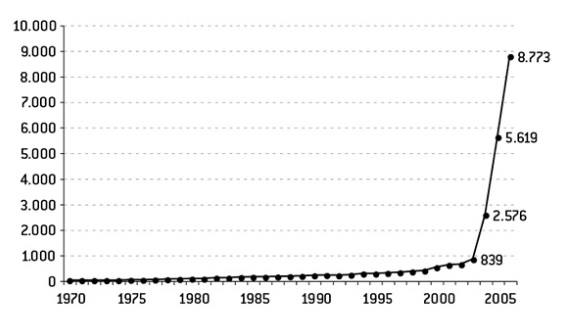
\includegraphics[scale=.5]{grafico}
	\caption{Número de participantes na Série Mundial de Pôquer entre 1970 e 2006}
\end{figure}

\end{frame}	

\section{Disposições gerais do Texas Hold'em}
\begin{frame}
\frametitle{Disposições gerais do \textit{Texas Hold'em}} 
Dentre todas as modalidades do pôquer a mais jogada é o \textit{Texas Hold'em}. Ele é praticado com um baralho tradicional de 52 cartas, em que nenhum naipe é superior ao outro e a sequência do valor das cartas se inicia com a carta de maior valor, isto é, o Ás até o menor valor, 2.

\end{frame}

\begin{frame}
\frametitle{Disposições gerais do \textit{Texas Hold'em}} 
\begin{center}
{\Large \textbf{Objetivo}}
\end{center}
O objetivo no \textit{Hold'em} é obter a melhor combinação entre as cartas pessoais e as cartas comunitárias. Cada jogador possui um total de fichas ao participar da partida, caso o montante pessoal acabe o jogador está fora do jogo, portanto o jogador vencedor é aquele que conquista todas as fichas.	

\end{frame}

\begin{frame}
\frametitle{Disposições gerais do \textit{Texas Hold'em}} 
\begin{center}
{\Large \textbf{Ranking das mãos}}
\end{center}
\begin{figure}[t]
	\centering
	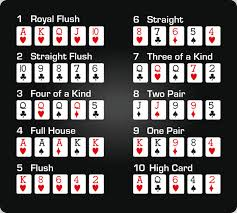
\includegraphics[scale=.7]{ranking2}
	\label{rakingmaos}
	\caption{Ranking das mãos do \textit{Texas Hold'em} por ordem decrescente}
\end{figure}

\end{frame}

\begin{frame}	
\frametitle{Disposições gerais do \textit{Texas Hold'em}} 
\begin{center}
{\Large \textbf{Ações}}
\end{center}
No \textit{Texas Hold'em} cada jogador pode realizar as seguintes ações: 
\begin{enumerate}
\item \textbf{Check/Mesa}
\item \textbf{Bet/Apostar}
\item \textbf{Call/Pagar} 
\item \textbf{Raise/Aumentar}
\item \textbf{Fold/Desistir}
\end{enumerate}	
	
\end{frame}

\begin{frame}	
\frametitle{Disposições gerais do \textit{Texas Hold'em}} 
\begin{center}
{\Large \textbf{Rodadas}}
\end{center}
No \textit{Texas Hold'em} há quatro rodadas: 
\begin{enumerate}
\item \textbf{Pré-Flop}
\item \textbf{Flop}
\item \textbf{Turn}
\item \textbf{River}
\end{enumerate}	

\end{frame}


\section{Cálculo do Flush através do modelo Hipergeométrico}
\begin{frame}
\frametitle{Cálculo do Flush através do modelo Hipergeométrico} 
\begin{itemize}
	
\item Para que jogadores de pôquer tenham um bom desempenho no jogo é preciso que conheçam a probabilidade de obter cada mão de forma rápida e objetiva.

\item O flush, uma das mãos do pôquer, é formado pela combinação de cinco cartas do mesmo naipe. Estamos interessados na probabilidade de sair 3 ou 4 cartas do mesmo naipe (dependendo da mão).
\end{itemize}
\end{frame}

\begin{frame}
\frametitle{Cálculo do Flush através do modelo Hipergeométrico} 
\begin{center}
	{\Large \textbf{Flush}}
\end{center}

\begin{figure}[h]
	\centering
	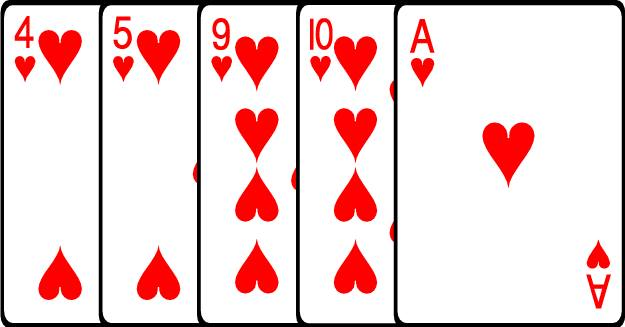
\includegraphics[scale=.4]{flush}
	\label{rakingmaos}
	\caption{\textit{Flush} de Ás}
\end{figure}
\end{frame}

\begin{frame}
\frametitle{Cálculo do Flush através do modelo Hipergeométrico}
\begin{center}
	{\Large \textbf{Distribuição hipergeométrica}}
\end{center}

A variável aleatória $X$ segue uma distribuição hipergeométrica se sua função de probabilidade é dada por: 

\begin{equation}\label{hip}
	P(X = k) = \dfrac{\binom{R}{k}\,\binom{N - R}{n - k}}{\binom{N}{n}}
\end{equation}

em que,
\begin{itemize}
	\item $N$ é o tamanho da população;
	\item $R$ é o número de sucessos dentro população;
	\item $n$ é o número de ensaios;
	\item $k$ é o número de sucessos observados.
\end{itemize}

\end{frame}

\begin{frame}
\frametitle{Cálculo do Flush através do modelo Hipergeométrico}
Dessa maneira se definirmos $X = $ \textbf{número de cartas de um certo naipe que formam um flush}, então $X$ segue um distribuição Hipergeométrica, porém o parâmetro $R$ depende das cartas pessoais.\\
\vspace{.2cm}
O número de ensaios ($n$), ou seja, número de cartas que irá aparecer é 5 e $N = 50$, pois há 52 cartas em um baralho, entretanto antes do flop conhecemos apenas as cartas pessoais.
\end{frame}
\begin{frame}
\frametitle{Cálculo do Flush através do modelo Hipergeométrico}	

\begin{center}
{\Large \textbf{Cartas pessoais de naipes distintos}}
\end{center}
Neste caso $R = 12$ e $k = 4$, fazemos ainda uma multiplicação por dois, pois estamos calculando o flush apenas para uma das cartas pessoais.

\begin{equation}
2\cdot P(X = 4) = 2\cdot\left[\dfrac{\binom{12}{4}\,\binom{50 - 12}{5 - 4}}{\binom{50}{5}}\right] = 2\cdot0.008877 = 0.017755
\end{equation}
\end{frame}

\begin{frame}
\frametitle{Cálculo do Flush através do modelo Hipergeométrico}
\begin{center}
{\Large \textbf{Cartas pessoais de naipes semelhantes}}
\end{center}
Quando há duas cartas de mesmo naipe o calculo é feito com $R = 11$ e $k = 3$.	

\begin{equation}
\displaystyle P(X = 3) = \dfrac{\binom{11}{3}\,\binom{50 - 11}{5 - 3}}{{50 \choose 5}} = 0.05770
\end{equation}

\end{frame}


\section{Outs, Odds e Pot Odds}
\begin{frame}
\frametitle{Outs, Odds e Pot Odds}
\begin{center}
	Outs: Cartas que melhoram a mão
	
	\begin{equation*}
	Odds = \frac{1 - Probabilidade\ de\ obter\ melhora}{Probabilidade\ de\ obter\ melhora}
	\end{equation*}
	
	\begin{equation*}
	Pot\ Odds = \frac{Pote\ da\ rodada}{Valor\ da\ aposta\ a\ ser\ paga}
	\end{equation*}
\end{center}
\end{frame}

\begin{frame}
	\frametitle{Outs, Odds e Pot Odds}
\begin{center}
{\Large \textbf{``Regra do 4 e 2''}}
\end{center}
A regra consiste em multiplicar o número de \textit{Outs} por 4 para saber a probabilidade de obter uma melhora no \textit{Turn} e/ou \textit{River}, e multiplicar por 2 para saber a probabilidade de obter a melhora somente na virada da próxima carta da mesa, o produto resultante é a porcentagem que representa a chance da melhora ocorrer.
\end{frame}

\begin{frame}
	\frametitle{Outs, Odds e Pot Odds}
	Exemplo: O jogador A, possui um \textit{Gutshot Straight} no \textit{Flop}, o oponente realiza uma aposta de \$20, aumentando o pote para \$280. O jogador A deve pagar ou desistir da aposta?
	\begin{itemize}
		\item Outs = 4
		\item $ P(Straight \mid Gutshot\ Straight) = 4 \cdot 2 = 8\%$
		\item Odds = $92\% \div 8\% \approx 11\%$
		\begin{center}
			Odds: 11 : 1
		\end{center}
		\item Pot Odds = $280 \div 20 = 14$
		\begin{center}
			Pot Odds: 14 : 1
		\end{center}
	\end{itemize}
\end{frame}

\begin{frame}{Outs, Odds e Pot Odds}
	A justificativa dessa decisão decorre principalmente do fato de que a longo prazo, o jogador resultará em lucros, pois, a cada 12 jogadas 11 delas o jogador não atingirá a melhora da mão, ocasionando possivelmente na perda da aposta paga, cujo valor é de \$20. Por outro lado, em 1 das 12 mãos o jogador irá obter a mão desejada, acarretando possivelmente na vitória do pote de \$280.
	\begin{center}
		$-11 \times \$20 + 1 \times \$280 = \$60$
	\end{center} 
\end{frame}

\section{Conclusão}
\begin{frame}
\frametitle{Conclusão} 
Portanto, no presente trabalho foram abordados os seguintes tópicos de maneira satisfatória:
	\begin{itemize}
		\item Apresentação sucinta da história do pôquer e o seu desenvolvimento
		\item No pôquer, é possível a aplicação de modelos probabilísticos, tal como o modelo hipergeométrico
		\item Existem métodos de tomada de decisão fundamentados em conceitos probabilísticos
	\end{itemize}
\end{frame}

\section{Referências}
\begin{frame}
\frametitle{Referências} 
	\begin{thebibliography}{5}
		\nocite{*}
		\bibitem{ross} ROSS, Sheldon. \textbf{A First Course in Probability}, 5ª edição, University of California, Berkeley, 1998.
		
		\bibitem{degroot} DEGROOT, Morris H; Schervish, Mark J. Expectation. In: \_\_\_\_\_\_. \textbf{Probability and Statistics}. 4 ed. Addison-Wesley, 2012. p. 207-273.
		
		\bibitem[silver] SSILVER, Nate. A bola do pôquer. In: \_\_\_\_\_\_. \textbf{O sinal e o ruído}. 1 ed. Rio de Janeiro. Editora Intrínseca, 2013. p 302-338;

		\bibitem[trevor] SSIPPETS, Trevor. \textbf{Guia prático do pôquer}. São Paulo : Editora Escala, 2010.
		
		\bibitem[adiga] LLEONARD, Tom. \textbf{Poker Drawing Odds \& Outs}. Disponível em: <http://www.pokerology.com/lessons/drawing-odds>. Acesso em: 17 set. 2015 .	
	\end{thebibliography}
\end{frame}

\end{document}